% =============================================================================
%  Two channels of a contact network: what the folded prime polymer remembers
%  Paper 4 of the PDTP series.  Draft 1, 2 October 2026.
%  Every number is produced by a script in ../scripts from the CSVs in ../data.
% =============================================================================
\documentclass[reprint,amsmath,amssymb,aps,pre,longbibliography]{revtex4-2}
\usepackage{graphicx}
\usepackage{bm}
\usepackage{amsthm}
\usepackage[colorlinks=true,linkcolor=blue,citecolor=blue,urlcolor=blue]{hyperref}
\graphicspath{{./figures/}}
\newtheorem{proposition}{Proposition}

\begin{document}

\title{Two-channel duality, fold memory, and arithmetic blindness\\
in polymer contact networks}

\author{Ruqing Chen}
\email{ruqing@hotmail.com}
\thanks{Archived at \href{https://doi.org/10.5281/zenodo.23100245}{doi:10.5281/zenodo.23100245}.}
\affiliation{GUT Geoservice Inc., Montreal, Quebec, Canada}
\date{\today}

\begin{abstract}
The contact network of a collapsed polymer is a finite graph, and graph invariants of the kind
used in algorithmic class field theory --- the Laplacian, its sandpile group, the discrete Hodge
decomposition, the Albanese metric of a periodic cover, the Perron branch of the adjacency ---
can be read off it exactly. We apply them to 82 conformations of the prime-driven topological
polymer (PDTP), whose bending stiffness follows the prime gaps, against surrogates that shuffle the
gaps (S1) or keep only their smooth prime-number-theorem envelope (S6$''$). Unweighted invariants,
including the exact sandpile group, do not distinguish the arms. The sequence enters through a
divisor, the rank of the stiffness on the vertices, and the two channels then separate. In the
bulk (Laplacian) channel the divisor energy $D^{\top}\Delta^{+}D$ separates the true chain from
its shuffles at $Z_{\rm seq}=+11.4$ in both partially collapsed and fully relaxed globules, while
the boundary (Perron) channel separates no pair of arms. The bulk channel reads the envelope: the
PNT-only surrogate matches the true chain ($p=0.76$), and once the smooth positional modes are
removed every arm contrast vanishes ($p_{\rm Holm}=1$ for all 16 envelope-removed tests). A
marginal true-versus-S6$''$ difference seen in an eight-globule pilot ($p=0.043$) does not
replicate on the full library. What survives in every channel and every arm is a strong memory of
the globule's own sequence, $z\approx6$ to $24$ against gap shuffles on the same conformation,
equal across arms. The folded network remembers its sequence, and the arithmetic it can tell apart
is the envelope's. Two textbook identities hold exactly on all 82 graphs: the backbone winding has
Albanese energy $N$, and the spanning-tree count times the closure-flux energy is an integer.
\end{abstract}

\maketitle

%==============================================================================
\section{Introduction}
%==============================================================================

A self-avoiding chain whose bending stiffness follows the gaps between consecutive primes (the
prime-driven topological polymer, PDTP) collapses into a globule that is measurably less radially
sorted than one built from a shuffle of the same gaps~\cite{PDTP4}. The imprint survives complete
relaxation; its correlation length is a property of the readout; and it is carried by the smooth
prime-number-theorem (PNT) envelope at the small-prime end of the chain~\cite{PDTP4,Merged}. A
companion study showed that no ordering, positional or scattering readout of the chain registers
congruence structure beyond sieve composition~\cite{Paper3}.

Every one of those readouts treats the conformation as a set of positions. A collapsed chain is
also a network: beads are vertices, bonds and contacts are edges. Contact maps are the primary data
of chromosome conformation capture~\cite{LiebermanAiden}, and the mathematics of finite graphs
offers invariants that see more than positions. The algorithmic class field theory of
Ref.~\cite{ANCCFT} organizes them into two channels. The \emph{bulk} channel is the Laplacian
$\Delta$, whose cokernel has the sandpile (critical) group as torsion~\cite{Biggs} and which, on
arithmetic quotients of the Bruhat--Tits tree, carries Frobenius traces. The \emph{boundary}
channel is the non-backtracking or adjacency operator, whose equilibrium states see only the Perron
branch of the spectrum. The first principle of Ref.~\cite{ANCCFT} is that the two channels do not
see the same thing: the boundary is arithmetically blind, the bulk is not.

Here we ask what the two channels of the PDTP contact network see of the prime sequence. A contact
network is not an arithmetic quotient, so the trace formulas of Ref.~\cite{ANCCFT} do not apply,
and we borrow its constructions, not its theorems. The answer has three parts. Unweighted
invariants see nothing of the sequence. Weighted by the sequence, the bulk channel sees the PNT
envelope and the boundary channel sees no arm difference. And beyond the envelope every channel
shows a memory of the globule's own sequence that is the same for primes, shuffles and
PNT-only surrogates.

%==============================================================================
\section{The contact network and its invariants}\label{sec:defs}
%==============================================================================

\emph{Graph.} For a conformation $\{\mathbf r_i\}_{i=0}^{N-1}$ the contact graph $Y$ has the
backbone bonds $(i,i+1)$ and the non-bonded contacts $|\mathbf r_i-\mathbf r_j|<1.5\sigma$,
$|i-j|>1$. Edges are oriented $i<j$; $d$ is the $N\times m$ incidence matrix with $d_{ie}=-1$,
$d_{je}=+1$, so that $(d^{\top}f)_e=f_j-f_i$ and $\Delta=dd^{\top}$ is the graph Laplacian. The
backbone makes $Y$ connected.

\emph{Bulk channel.} The sandpile group is ${\rm Jac}(Y)={\rm Tor}\,{\rm coker}\,\Delta$, of order
the number $\kappa(Y)$ of spanning trees, with structure read off the Smith normal
form~\cite{Biggs,ANCCFT}. A sequence enters as a degree-zero divisor on the vertices,
$D=\mathrm{rank}(k)-\overline{\mathrm{rank}(k)}$, with $k_i$ the bead stiffness. Its class in
${\rm Jac}$ has an order, and its energy in the Laplacian metric is
\begin{equation}
E(D)=D^{\top}\Delta^{+}D .
\label{eq:E}
\end{equation}

\emph{Envelope removal.} Let $P_{\le K}$ project onto the Legendre polynomials of degree $\le K$
in the backbone coordinate $x_i=2i/(N-1)-1$, orthonormalized on the grid. The envelope-removed
divisor is $D_K=D-P_{\le K}D$, and $E_K=E(D_K)$.

\emph{Hodge decomposition.} A 1-form $f$ on the edges splits orthogonally as
$f=d^{\top}\phi+h$ with $dh=0$: a gradient plus a cycle (harmonic) part~\cite{Lim,ANCCFT}. The
coboundary $d^{\top}k$ of any vertex function is a gradient, so its cycle part vanishes
identically on every graph. To obtain a sequence-sensitive cycle energy we use the stiffness-rank
difference carried by the contacts only, $f_e=\mathrm{rank}(k)_j-\mathrm{rank}(k)_i$ on contacts
and $f_e=0$ on the backbone, and report the cycle share $H_c=\|h\|^2/\|f\|^2$. Setting $f$ to zero on the backbone breaks the
exactness of the full coboundary: $f$ is no longer the gradient of any vertex function, and its
harmonic part is the projection of the sequence's stiffness contrast onto the cycle space. Every
cycle of $Y$ contains at least one contact, since the backbone alone is a tree, so this part
measures how the stiffness contrast circulates around the loops closed by long-range contacts.

\emph{Boundary channel.} We use the Perron vector $v_P$ of the adjacency matrix and the rank
correlation $\rho_P={\rm Spearman}(k,v_P)$.

\emph{Albanese energy.} Closing the chain by one edge $e^*=(0,N-1)$ gives a unit cell $Y^*$ for a
$\mathbb Z$-periodic lattice. For a winding cochain $\alpha$ the inverse effective mass of the band
bottom is $M^{-1}=(2t/n)\,\alpha^{\top}\Pi\alpha$, with $\Pi=I-d^{*\top}\Delta^{*+}d^*$ the
projector onto the cycle space~\cite[Ch.~22]{ANCCFT}.
\begin{proposition}\label{prop:alb}
(i) For the backbone winding, $\alpha=$ the indicator of the ring, $\alpha^{\top}\Pi\alpha=N$ for
every conformation. (ii) For the closure flux, $\alpha=$ the indicator of $e^*$,
$\alpha^{\top}\Pi\alpha=1/(1+R)$, with $R$ the effective resistance between the two chain ends in
the open graph $Y$. (iii) $\kappa(Y^*)/(1+R)=\kappa(Y)$ is an integer.
\end{proposition}
\begin{proof}
(i) The ring is a cycle, so $\Pi\alpha=\alpha$ and the energy is its length~\cite[Cor.~22.4.3]{ANCCFT}.
(ii) $\alpha^{\top}\Pi\alpha=1-R^{Y^*}(e^*)$~\cite[Thm.~22.4.1]{ANCCFT}, and $e^*$ in parallel with
$Y$ gives $R^{Y^*}(e^*)=R/(1+R)$~\cite{KleinRandic}. (iii) $1-R^{Y^*}(e^*)=\kappa(Y^*-e^*)/\kappa(Y^*)$
by Kirchhoff's theorem, and $Y^*-e^*=Y$.
\end{proof}
\noindent The backbone winding therefore carries no information about the conformation, and the
closure flux reduces to the end-to-end resistance of the contact network. Written for the inverse
effective mass, (iii) reads $\kappa(Y^*)\,(n/2t)\,M^{-1}=\kappa(Y)$. Multiplying the closed
network's inverse effective mass, in its natural unit, by the spanning-tree count of the closed
network returns exactly the spanning-tree count of the open one. The band curvature is therefore
quantized in units of $2t/[n\,\kappa(Y^*)]$, the discrete-topological quantization of
Ref.~\cite[Cor.~22.4.2]{ANCCFT}. It is an identity of Kirchhoff type, valid for every graph, and
the exact checks of Sec.~\ref{sec:results} test the computation, not the physics.

%==============================================================================
\section{Data and statistics}\label{sec:data}
%==============================================================================

We use the 82 stored conformations of PDTP~v4.0~\cite{PDTP4} at $N=4\times10^4$. The
\emph{production} globules are partially collapsed coils after an 8000-step anneal: 24 of the true
chain, 8 S1 shuffles and 40 S6$''$ surrogates (exact gap multiset arranged as a PNT scale family,
with no prime-specific fluctuation). The \emph{relaxed} globules are melt-density globules after a
$10^6$-step isothermal hold~\cite{Merged}: 5 true, 5 S1. The production graphs have
$7.6$--$7.9\times10^4$ contacts; the relaxed graphs $1.88\times10^5$. All 82 conformations are used in every analysis below.

\emph{Own-sequence null.} For every globule and every sequence-weighted statistic we compute the
same statistic for 20 random permutations of the globule's own gaps, placed on the same
conformation, and report $z=(x-\bar x_{\rm null})/s_{\rm null}$. A large $z$ means that the
conformation is adapted to its own sequence.

\emph{Arm contrasts.} The true arm is one fixed sequence; each surrogate globule has its own
sequence. Following PDTP~v4.0~\cite{PDTP4} we use a sequence-level statistic,
$Z_{\rm seq}=(\bar x_T-\bar x_S)/[\hat\sigma^2_{\rm seq}+s_T^2/n_T+s_S^2/n_S]^{1/2}$, with the
thermal variance estimated from the true arm and
$\hat\sigma^2_{\rm seq}=\max(0,s_S^2-s_T^2)$, referred to $t_{n_S-1}$. Holm~\cite{Holm} and
Benjamini--Hochberg~\cite{BH} corrections are applied within each family of tests.

%==============================================================================
\section{Results}\label{sec:results}
%==============================================================================

\subsection{Unweighted invariants are blind}
We computed eight invariants that do not use the sequence directly on all 82 graphs: the mean
degree ($5.8$--$6.0$ in production, $11.4$ relaxed), $\ln\kappa$ ($5.5$--$5.6\times10^4$ and
$9.22\times10^4$), the algebraic connectivity, the adjacency spectral radius, and, on 400-vertex
coarse-grained graphs (blobs of 100 beads), the exact sandpile group computed with PARI/GP: its
order ($10^{363}$--$10^{374}$ in production, $10^{558}$--$10^{563}$ relaxed), its 2- and 3-ranks,
and the order of the sequence divisor in it. Of the 32 sequence-level contrasts (eight invariants,
four pairs of arms) the smallest uncorrected $p$ is $0.032$, and every Holm-adjusted $p$ equals 1.
The divisor's order is within a factor $10^{0.2}$--$10^{0.5}$ of the group exponent in every arm,
the same as for the globule's own gap shuffles ($10^{0.1}$--$10^{0.6}$). The arithmetic of
${\rm Jac}(Y)$ does not record the sequence.

\subsection{The bulk channel reads the envelope}
The divisor energy, Eq.~\eqref{eq:E}, is the first sequence-sensitive invariant
(Fig.~\ref{fig:bulk}, Table~\ref{tab:bulk}). In the production globules the true chain lies far
above its own shuffles ($z=+33.5$) and so does S6$''$ ($+28.9$), while S1 barely does ($+2.6$). At
the sequence level the true chain separates from S1 ($Z_{\rm seq}=+11.4$) and from nothing else: it
matches S6$''$ ($Z_{\rm seq}=+0.31$, $p=0.76$). The relaxed globules repeat the true-versus-S1
separation ($Z_{\rm seq}=+11.4$). The channel reads the composition profile along the chain, the PNT
envelope, which S6$''$ shares and S1 destroys.

The mechanism is quantitative. The Legendre modes up to degree 4 carry $2.9\%$ of $\|D\|^2$ for the
true chain, $2.5\%$ for S6$''$ and $0.2\%$ for S1. Because $\Delta^{+}$ weights each mode by the
inverse of its eigenvalue, and the backbone makes chain-scale profiles the softest modes of the
network, this small fraction dominates the energy.

\begin{figure*}[t]
\centering
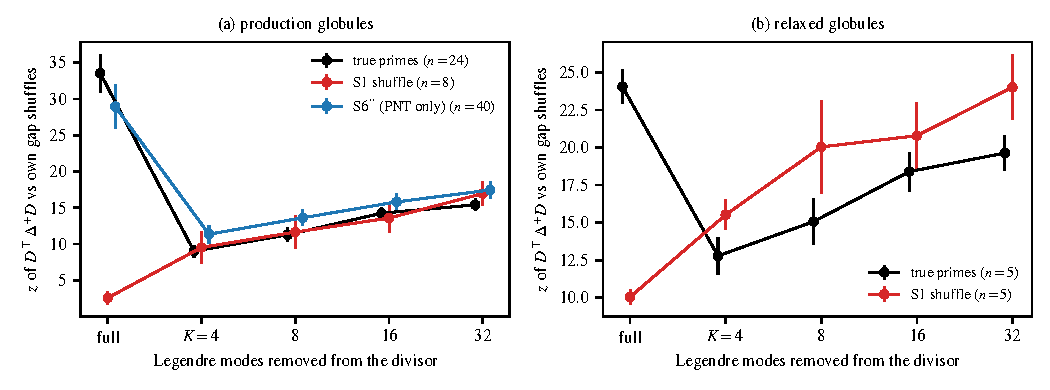
\includegraphics[width=\linewidth]{fig1_bulk_channel.pdf}
\caption{Bulk channel. $z$ of the divisor energy against each globule's own gap shuffles (mean
$\pm$ s.e.m.), for the full divisor and with Legendre modes up to degree $K$ removed.
(a)~Production globules; (b)~relaxed globules. The full divisor separates the envelope-carrying
arms (true, S6$''$) from S1; removing the smooth modes removes every arm difference.}
\label{fig:bulk}
\end{figure*}

\begin{table}[t]
\caption{Sequence-level contrasts of the divisor-energy $z$ (Fig.~\ref{fig:bulk}). Full: $K=0$.
Envelope-removed: the four tests $K\in\{4,8,16,32\}$; range of $p_{\rm seq}$, and Holm-adjusted
$p$ over all 16 envelope-removed tests.}
\label{tab:bulk}
\footnotesize
\begin{ruledtabular}
\begin{tabular}{llrrrr}
 & & \multicolumn{2}{c}{full} & \multicolumn{2}{c}{envelope removed}\\
protocol & contrast & $Z_{\rm seq}$ & $p_{\rm seq}$ & $p_{\rm seq}$ & $p_{\rm Holm}$\\ \hline
production & true $-$ S1 & $+11.35$ & $9\times10^{-6}$ & 0.63--0.94 & 1\\
production & true $-$ S6$''$ & $+0.31$ & 0.76 & 0.67--0.81 & 1\\
production & S6$''$ $-$ S1 & $+8.35$ & $7\times10^{-5}$ & 0.38--0.82 & 1\\
relaxed & true $-$ S1 & $+11.40$ & $3\times10^{-4}$ & 0.16--0.65 & 1\\
\end{tabular}
\end{ruledtabular}
\end{table}

\subsection{Nothing survives envelope removal}
Removing the Legendre modes up to degree $K=4$, $8$, $16$ or $32$ removes every arm contrast
(Table~\ref{tab:bulk}). None of the 16 envelope-removed tests reaches $p_{\rm seq}<0.15$, and after
correction all have $p_{\rm Holm}=1$ and $p_{\rm BH}=0.94$. In particular, an eight-globule pilot had
shown the true chain above S6$''$ at $K=16$ ($p=0.043$ uncorrected, Welch). On the full library of 24
true and 40 S6$''$ globules the difference has the opposite sign ($z=+14.3$ against $+15.8$) and
$p_{\rm seq}=0.81$. The pilot was a fluctuation. The large between-sequence spread of the S6$''$
class ($\hat\sigma_{\rm seq}\approx6$ in $z$) shows why: a handful of surrogate sequences cannot
fix the class mean.

\subsection{The boundary channel separates no arms}
The Perron correlation $\rho_P$ is also far from its own-sequence null, with the opposite sign
($z=-3.5$, $-3.2$, $-5.0$ for true, S1 and S6$''$ in production; $-10.4$ and $-12.9$ relaxed), but
it does not distinguish the arms: no contrast survives correction (smallest $p_{\rm Holm}=0.16$).
The two-channel dichotomy of Ref.~\cite{ANCCFT} therefore has a polymer counterpart: the bulk sees
the envelope and the boundary does not. Neither sees anything beyond the envelope.

\subsection{Every channel remembers the globule's own sequence}
Figure~\ref{fig:memory} collects the own-sequence $z$ of four statistics. All are far outside the
null band in every arm. The envelope-removed divisor energy has $z\approx14$ to $21$; the contact
cycle share $H_c$, whose values are $0.053$--$0.055$ in production and $0.035$ relaxed, has
$z\approx6$ in production and $8$--$11$ relaxed; the Perron correlation has $z\approx-3$ to $-13$.
None separates the arms after correction (cycle share: smallest $p_{\rm Holm}=0.56$, relaxed true
versus S1).

The conformation is thus strongly adapted to its own stiffness sequence: stiff and flexible
segments find contacts that a random rearrangement of the same gaps would not give them. That
adaptation is the generic physics of a semiflexible collapse. A shuffled sequence folded by the
same dynamics is adapted to itself just as strongly. It is memory of the sequence, not of
arithmetic.

\begin{figure*}[t]
\centering
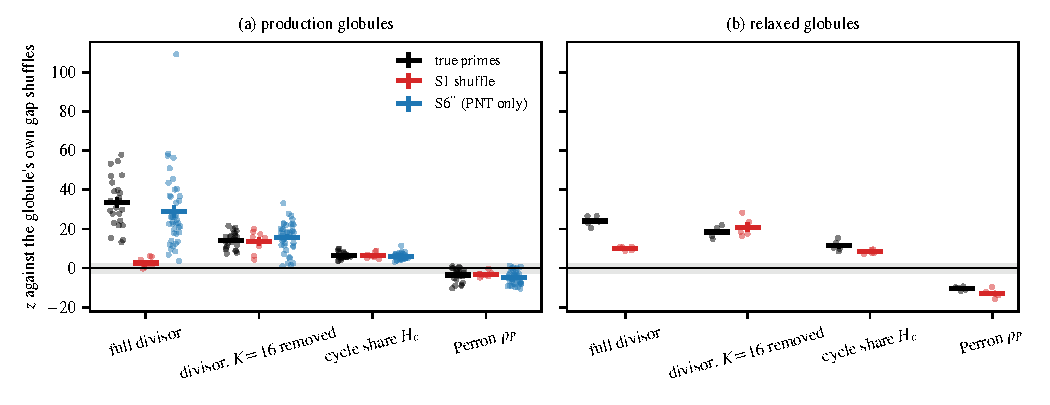
\includegraphics[width=\linewidth]{fig2_memory.pdf}
\caption{Own-sequence memory. Per-globule $z$ against 20 gap shuffles on the same conformation,
for the full divisor energy, the envelope-removed divisor energy ($K=16$), the contact cycle share
$H_c$ and the Perron correlation $\rho_P$ (dots: globules; bars: mean $\pm$ s.e.m.; grey: $|z|<2$).
(a)~Production; (b)~relaxed. Panel (b) has no S6$''$ arm because the $10^6$-step isothermal hold was
run only for the true chain and the S1 shuffle~\cite{Merged}.}
\label{fig:memory}
\end{figure*}

\subsection{Albanese energies and exact checks}
Proposition~\ref{prop:alb} holds on all 82 graphs: the backbone winding has energy exactly $N$, and
on the coarse graphs $\kappa(Y^*)/(1+R)$ is an integer in 82 of 82 cases (PARI/GP, exact
arithmetic). The closure flux reduces to the end-to-end resistance $R$ (Fig.~\ref{fig:alb}). In
the relaxed globules $R=0.32\pm0.17$ (true) and $0.30\pm0.07$ (S1), indistinguishable. In the
partially collapsed production globules $R$ spans more than two decades and its median is lower
for the true chain than for S1, but no contrast survives correction (smallest $p_{\rm Holm}=0.16$,
S6$''$ versus S1). The effective mass of the closed network is set by how well its two ends are
connected, which is a property of the collapse, not of the sequence.

\begin{figure}[t]
\centering
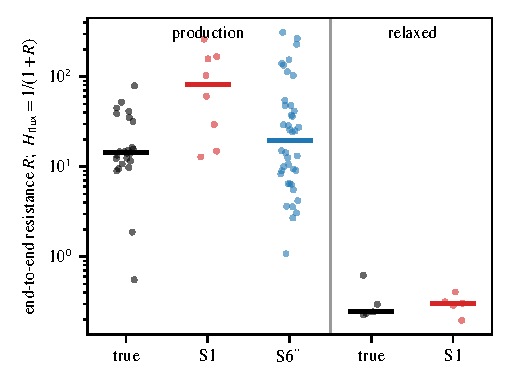
\includegraphics[width=\linewidth]{fig3_closure_flux.pdf}
\caption{End-to-end effective resistance $R$ of the contact network (log scale; bars: medians).
The closure-flux Albanese energy is $1/(1+R)$ (Proposition~\ref{prop:alb}).}
\label{fig:alb}
\end{figure}

%==============================================================================
\section{Discussion}\label{sec:disc}
%==============================================================================

The constructions of algorithmic class field theory transfer to the contact network of a folded
polymer and are exactly computable on it, but the arithmetic content that makes them interesting
on arithmetic quotients does not transfer with them. On the Bruhat--Tits tree the sandpile order
is a product of Frobenius traces and the bulk channel carries automorphic data~\cite{ANCCFT}. On a
contact network the sandpile group is a large, generic abelian group whose structure does not
depend on the sequence that drove the collapse. What the bulk channel registers is the sequence
\emph{as a function on the vertices}, through the energy of a divisor. That energy is dominated by
the chain-scale modes, which for the primes are the PNT envelope.

The two-channel picture nevertheless survives in a reduced form. The bulk channel separates the
envelope-carrying arms from the shuffle; the boundary channel separates nothing. This is the
dichotomy of Ref.~\cite{ANCCFT} with its arithmetic content replaced by positional content, and it
matches the conclusion of the companion paper: polymer readouts see the arithmetic of a prime
sequence through its envelope and its composition, and through nothing finer~\cite{Paper3}. The
eight-globule pilot that suggested otherwise did not replicate, and we report it as a cautionary
example of how a random-effects design and a family-wise correction change the reading of a
marginal $p$-value.

What every channel does see is memory. A collapsed globule is adapted to its own stiffness
sequence: its contacts, cycles and Perron mode are all far from what the same conformation would
give a permuted sequence. This is a property of folding, not of the primes, and it is equally
strong for shuffles. It may be useful elsewhere. For contact maps measured in experiment, the
own-sequence $z$ of a divisor energy is a parameter-free measure of how strongly a conformation is
adapted to a sequence-dependent property of its monomers.

\emph{The series in one picture.} This paper closes a four-part study of what a polymer folded
under a prime-programmed stiffness can register of the primes~\cite{PDTP4,Merged,Paper3}. The
picture it leaves is simple. The fold has a strong topological memory of its own sequence: its
radial organization, its contacts, its cycles and its Perron mode are all adapted to the stiffness
sequence that drove the collapse. That memory is generic, as strong for a random permutation of
the gaps as for the primes. Its response to number-theoretic detail is confined to two channels:
the smooth prime-number-theorem envelope, read through the position of each bead along the chain,
and the sieve composition of the gap multiset, which converges with sieve depth. Correlation
lengths that grow with the chain, congruence confinement, and every finer arithmetic structure we
tested lie outside what the fold reads.

\emph{Limitations.} The contact graph depends on the cutoff $r_c$, which we did not vary. The
production globules are partially collapsed coils, and only ten relaxed globules exist. The S1 arm
has eight production globules. Exact sandpile arithmetic is computed only on coarse-grained graphs.
The S6$''$ surrogate matches the leading Legendre coefficients of the true composition to
$0.93$--$1.0$~\cite{PDTP4}, so residual envelope differences at the few-percent level cannot be
excluded at $K\le4$; at $K\ge8$ they are removed by construction.

%==============================================================================
\section{Conclusion}
%==============================================================================

On 82 conformations of a prime-programmed polymer, the invariants of the contact network fall into
three groups. Unweighted invariants, including the exact sandpile group, are blind to the
sequence. Sequence-weighted bulk invariants see the prime-number-theorem envelope, and boundary
invariants see no arm difference: the two-channel dichotomy of algorithmic class field theory,
with positional in place of arithmetic content. Every channel records a strong memory of the
globule's own sequence that is identical for primes, shuffles and PNT-only surrogates. Nothing in
the contact network distinguishes the primes from a smooth model of their density once the
envelope is removed; a marginal pilot signal to the contrary did not replicate.

\begin{acknowledgments}
Code, data, tests and figure scripts are available at
\url{https://github.com/Ruqing1963/contact-network-two-channels} and archived at
\href{https://doi.org/10.5281/zenodo.23100245}{doi:10.5281/zenodo.23100245}. The conformations are those of
the PDTP repository, version~4.0~\cite{PDTP4}.
\end{acknowledgments}

\bibliography{references}

\end{document}
